%\mychapter{4}{Dimensionality Reduction}

\subsection{Dimensionality reduction}
In this section, we review some linear and non-linear dimensionality reduction techniques. We focus on spectral dimensionality reduction methods where the low dimensional model is obtained from spectral decomposition of an $n \times n$ positive semidefinite (PSD) proximity matrix (see appendix \ref{SVD} and \ref{proximity}). We start by defining dimensionality reduction and outline steps of spectral dimensionality reduction. Next give a brief description of PCA and the diffusion maps algorithm. In later sections, we compare the performance of PCA and diffusion maps on our spike train data set.\\

Let $\textbf{X} = \displaystyle \{\vect{x}_{1}, \ldots , \vect{x}_{n} \}$
be a set of $n$ data points, each of which is associated with $N$ features, so that each $\vect{x}_{i}$ is a point in a high dimensional space $\R^{N}$. Assume that the data points lie on or near an underlying $l$-dimensional manifold embedded in the high dimensional space where $l$ is much smaller than $N$. Dimensionality reduction considers the problem of  transforming the high dimensional data set
$\textbf{X}$ into a new data set $\textbf{Y} = \displaystyle \{ \vect{y}_{1}, \ldots, \vect{y}_{n} \}$  of $n$ points, each of which is associated
with a smaller set of $l$ features and such that each $\vect{y}_{i} \in \R^{l}$ is a low dimensional representation of $\vect{x}_{i} \in \R^{N}$ in the low dimensional space. In addition the transformation must preserve, as much as possible, the underlying geometry of the data.\\

Let $\Bm{X} \in \R^{n \times N}$ be a matrix of $n$ data points in a high dimensional space $\R^{N}$. Spectral dimensionality reduction (SDR) refers to all
dimensionality reduction methods which obtain a low dimensional model of $\Bm{X}$
by carrying out four main steps \cite{Lawrence2010}.
\begin{itemize}
\item[i)] A distance $d_{ij} = \text{dist}(x_{i}, x_{j})$, between data points
is chosen and a real number $l, 1 \leq l < N$ representing the desired dimensionality is fixed.
\item[ii)] From the distance, an $n \times n$ PSD proximity matrix  is computed.
\item[iii)] Spectral decomposition is carried out on the generated PSD matrix and
the top $l$ eigenvectors $\{ \vect{v}_{1}, \ldots, \vect{v}_{l} \}$ of the proximity matrix
form the columns in a new matrix, $\Bm{V} = [\vect{v}_{1}, \ldots, \vect{v}_{l}] \in \R^{n \times l}.$
\item[iv)] Viewing the $i^{th}$ row of $\Bm{V}$ as a point $\vect{y}_{i}$
in $\R^{l}$, a new set of $n$ points 
$\{\vect{y}_{1}, \ldots, \vect{y}_{n} \}$ is obtained such that each
 $\vect{y}_{i} = (\vect{v}_{1}(i), \ldots, \vect{v}_{l}(i)) \in \R^{l}$
is a low dimensional representation of $\vect{x}_{i} \in \R^{N}$.
\end{itemize}


\subsubsection{Linear dimensionality reduction}
Let $\Bm{X} \in \R^{n \times N}$ be a matrix of $n$ data points in a high dimensional space $\R^{N}$. Linear dimensionality reduction refers to the problem of finding a low dimensional model using a linear transformation of the data. The low dimensional model of the data $\Bm{Y}$, is obtained using the relation $\Bm{Y} = \Bm{M}^{\top}\Bm{X}$ where $M$ is an $n \times l$ matrix with $l \ll N$. A common spectral linear approach is principle component analysis (PCA) \cite{JolliffeIT1986PCAa}. PCA is a linear technique for finding the directions of maximum variance in the data. The main assumption in PCA is that the high dimensional data lie on or near a low $l$-dimensional linear subspace embedded in some high dimensional space $\R^{N}$. 
The low dimensional model that describes the data is found via spectral decomposition of the sample covariance matrix as follows:

\begin{itemize}
\item[i)] Compute the mean $\textbf{c}$ of the data set $\textbf{X}$ and center
the data so that $\textbf{X} = \textbf{X} - \textbf{c}.$
\item[ii)] Summarize the correlation relationships between the zero-mean data points by computing the sample covariance matrix $\frac{1}{n}\textbf{XX}^{\top}.$
\item[iii)] Find the spectral decomposition of $\textbf{XX}^{\top}$ or 
use SVD to find $\textbf{X} = \bm{U\Sigma V^{\top}}$  (see appendix \ref{SVD}).
\item[iv)] Let $\bm{V}_{l}$ denote the top $l$ columns of $\textbf{V}$ corresponding to the  top $l$ singular values of $\textbf{X}$.
\item[v)] The low dimensional model $\textbf{Y}$ is obtained by setting 
$\textbf{Y} = \textbf{V}^{\top}\textbf{X}$.
\end{itemize}

\subsubsection{Non-linear dimensionality reduction}

Methods like PCA assume that the underlying manifold on which the data lie is globally linear. This implies that the shortest distance between any two points on the manifold is a straight line.
However, any dimensionality reduction technique must preserve the underlying geometry of the data manifold. In particular, points that are close together in the high dimensional space should be mapped closer to each other in the low dimensional space where as points that are far apart in the high dimensional space must remain far apart in the embedded space. This idea of preserving distances between points is based on the multidimensional scaling (MDS) approach.
Figure \ref{fig:Swiss roll} illustrates the limitations of linear techniques on highly curved manifolds like the swiss roll and helps to highlight the importance of non-linear dimensionality reduction techniques.

\begin{figure}[h]
\centering
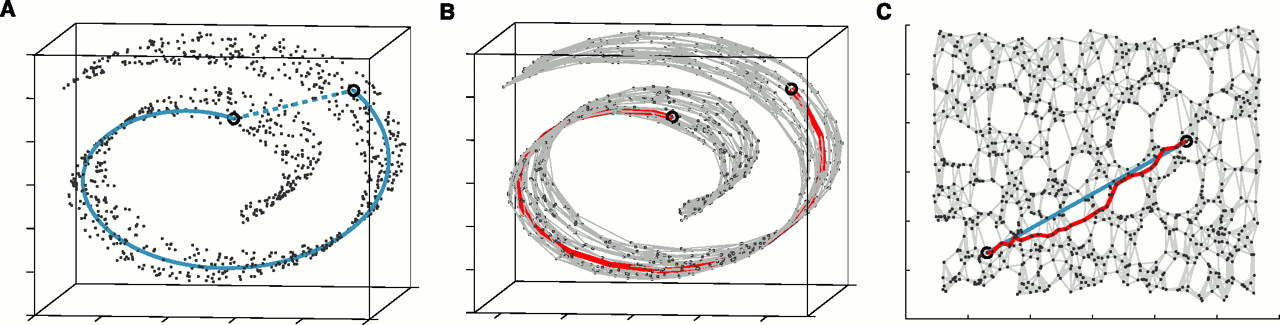
\includegraphics[width=\textwidth]{/home/tesylvia/Oral_Sept_2017/images/SwissRoll.jpg}
%label the figure so latex can reference it
\caption{ISOMAP on a swiss roll, taken from \cite{TenenbaumJB2000Aggf}}
      \label{fig:Swiss roll}
\end{figure}



(I need to explain what the figures in A-C mean based on the authors paper).


\subsubsection{Multidimensional scaling (MDS)}
Assume that an $n\times n$ matrix, $\Bm{B}$=(b$_{ij}$), of pair-wise distances
(not necessarily Euclidean) or similarities (see appendix \ref{proximity}), $\Bm{S} = (s_{ij})$, between data points, $\{\vect{x}_{1}, \ldots, \vect{x}_{n} \}$, is given (not the actual data points) and $n$ is large.
Multidimensional scaling (MDS) \cite{CoxT2000, MardiaK.V1979Ma} considers the the problem of finding a low dimensional model of the high dimensional data by searching for a configuration of $n$ points $\{\vect{y}_{1}, \ldots, \vect{y}_{n} \}$ in $\R^{\text{l}}, \text{l} \ll \text{n}$, where each $\vect{y}_{i}$ is a low dimensional representation of $\vect{x}_{i}$, and such that the pair-wise distances between points are preserved. Specifically, the Euclidean distances between the configuration points, $\norm{\vect{y}_{i} - \vect{y}_{j}}_{2}$, must be as ``close" as possible to  the given distances, d$_{ij}$, that is, $\norm{\vect{y}_{i} - \vect{y}_{j}}_{2} \approx \text{d}_{ij}$, for all $1 \leq i, j \leq n$.


\subsubsection{Key graph theory concepts}
The non-linear dimensionality reduction algorithms we consider are based on graph theory. Hence, we first introduce three key graph theory concepts that we need: weighted undirected graph, degree matrix and the graph Laplacian.\\
A graph is a tuple $G = (V,E)$ where $V = \{v_1, \ldots , v_n\}$ is a finite set of points called vertices or nodes and $E$ is a finite collection of edges connecting pairs of vertices. The graph $G$, is undirected if the edges between vertices are bidirectional.
We can make a weighted graph by assigning a weight or number $w_{ij}$, to an edge $e_{ij} \in E$, between a pair of vertices $(v_i, v_j) \in V$. A connectivity matrix or similarity matrix $\Bm{W}$, of $G$, is the matrix whose $(i,j)$-th entries are edge weights $w_{ij}$.
The degree $d_i$, is the sum of weights $w_{ij}$, of all edges connected to a vertex $v_i \in V$.
A diagonal matrix $\Bm{D}$, with degrees, $d_{i}$, on its diagonal is called the degree matrix.
The unnormalized graph Laplacian is the  matrix $\Bm{L = D} - \Bm{W}$.

   
 \subsubsection{Spectral non-linear dimensionality reduction}
Spectral non-linear dimensionality reduction (SNLDR) techniques are a 
class of MDS methods which find a low dimensional model of the data by preserving distances between neighboring points on a data manifold. These are the non-linear dimensionality
reduction algorithms that we will consider. Examples of SNLDR methods include ISOMAP \cite{TenenbaumJB2000Aggf}, locally linear embedding (LLE)  \cite{roweis2000nonlinear}, Laplacian eigenmaps (LE) \cite{belkin2003laplacian} and diffusion maps \cite{coifman2006diffusion}, in addition to many others. Unlike linear dimensionality reduction techniques, SNLDR methods do not make apriori assumptions about the underlying geometry of the data manifold.
SNLDR methods model local neighborhood relations between data points by building a graph on the data  \cite{Luxburg2007}. We only review the diffusion maps algorithm.


\subsubsection{Neighborhood graph}
Suppose we are given a data set, $\Bm{X} =  \{x_{1}, \ldots, x_{n} \}$ and assume that the pairwise distances, $d_{ij} = \text{dist}(x_{i}, x_{j})$, between points are known. Identifying each data point with a vertex $v_{i}$, on a graph $G = (V, E)$, we can build a weighted  undirected graph on the data where an edge $e_{ij} \in E$, between neighboring vertices $(v_i, v_j) \in V$, is weighted by a similarity measure $s_{ij}$, derived from the given distances.
The similarities, $s_{ij}$, are assigned such that points which are close together have a high similarity while points that are far apart have a low similarity. These pairwise similarities are used to model local neighborhood relations between input points and to obtain the graph Laplacian.
The eigenvectors of the graph Laplacian then provide a new coordinate system, which is used to embed the data into Euclidean space.\\


Given a data point $x_i \in \Bm{X}$, define $N_{\epsilon}(x_i) = \{x_j \in \Bm{X} \ \ | \ \ d(x_i, x_j) < \epsilon \}$. For each $x_j \in N_{\epsilon}(x_i)$, add an edge $e_{ij}$, to a graph $G$,
and assign that edge a similarity $s_{ij}$. Then in terms of the graph, the neighborhood
of $x_i$ consists of all vertices to which $x_i$ is connected.\\ 

There are two common methods for building neighborhood graphs:
One method is the $\epsilon-$nearest neighbor graph formed by connecting all points which are within a fixed distance $\epsilon$, from each other. Another method is the mutual $k$-nearest neighbor graph where two points $x_{i}$, and $x_{j}$, are connected together if and only if, $x_{i}$, is among the $k$-nearest neighbors of $x_{j}$, and $x_{j}$, is among the $k$-nearest neighbors of $x_{i}$, based on the chosen distance measure.


\subsubsection{Basic idea of diffusion maps algorithm}







%%%%%%%%%%%%%%%%%%%%%%%%%%%%%%%%%%%%%%%%%%%%%%%%%%%%%%%%%%%%%%%%%%%%%%%%%%%%%%%%%%%%%%%%%%%
%%%%%%%%%%%%%%Laplacian Eigen Maps algorithm %%%%%%%%%%%%%%%%%%%%%%%%%%%%%%%%%%%%%%%%%%%%%%
%\subsubsection{Laplacian eigen maps algorithm}
%Building a Graph from a data set $X = \{\vec{x}_{1}, \ldots , \vec{x}_{n}\}$}
%\pause
%Assuming the pairwise distances $d_{ij}$ or similarities $s_{ij}$ between data points $\{x_{1}, \ldots, x_{n}\}$
%are known, the points may be connected using 
%
%mutual k-nearest neighbor graph
%
%
%Build a weighted graph on the given data set
%by viewing data points as vertices of a graph in which neighboring points are connected by weighted edges
%
%From the adjacency matrix W  using one of the two methods
%
%Choose the weights $w_{ij}$ using the Heat Kernel with no parameter
%\[
% w_{ij} =
%  \begin{cases} 
%      \hfill e^{-\frac{\norm{\vec{x}_{i}-\vec{x}_{j}}^2}{t}}    \hfill & \text{ if $(i,j) \in E$} \\
%      \hfill 0 \hfill & \text{otherwise} \\
%  \end{cases}
%\]
%\pause
%
%\item Case 2: (No Parameter t).
%
%\[
% w_{ij} =
%  \begin{cases} 
%      \hfill 1    \hfill & \text{ if $(i,j) \in E$} \\
%      \hfill 0 \hfill & \text{otherwise} \\
%  \end{cases}
%\]
%
%
%
%
%
%and degree matrix D,
%compute the graph Laplacian L using the relationship L = D-W
%
%Solve the generalized eigenvalue problem Lv = $\lambda$Dv
%and stack the smallest  eigenvectors $\{\vec{v}_{1}, \ldots, \vec{v}_{d} \}$ of L excluding the smallest eigenevector of L as columns in a matrix U ;
%obtain a d-dimensional embedding of the data
% by viewing each  data point as the $i^{th}$ row of U via the map
%$\vec{x}_{i} \mapsto (\vec{v}_{1}(i), \ldots, \vec{v}_{d}(i))$ };
%
%
%
%
%
%
%\item Solve the generalized eigenvalue problem $L\vect{v} = \lambda D \vect{v}$ and take the bottom d-smallest generalized eigenvectors $\vect{f}_{2}, \ldots, \vect{f}_{d}$ of L excluding the constant eigenvector.
% \pause
% \item Form the matrix U = $[\vect{f}_{2} \ldots \vect{f}_{d}]$ by stacking $\vect{f}_{i}$ as columns in U.
% \pause 
% \item View the $\text{i}^{th}$ row of U as the $d$-dimensional representation of the $\text{i}^{th}$ vertex 
% corresponding to the original data point $\vect{x}_{i}.$
%




























